\documentclass[french, 12pt]{article}%


\usepackage[T1]{fontenc}
\usepackage[utf8]{inputenc}
\usepackage[french]{babel}

\usepackage{textcomp}

\usepackage[official]{eurosym}

\usepackage{appendix}
\usepackage{pdfpages}

%%%%%%%%%%%%%%%%%%%%%%%%%%%%%%%%%%%%%%%%%%%%%%%%%%%%%%%%%
\newcommand{\itemE}{\item[$\bullet$]}

\newcommand{\titreSeq}{Gestion des logs}
\newcommand{\lycee}{Académie rennes}
\newcommand{\classSeq}{CIEL }
\newcommand{\matiereSeq}{IR}      
\newcommand{\numSeq}{Cyber}
\newcommand{\numAct}{05}
\newcommand{\objSeance}{Comment gérer les logs}

\newcommand{\moySeq}{\begin{itemize}	
\itemE VM serveurCyber
\end{itemize}}


\newcommand{\paraL}[1]{\tiny\noindent\rule{1.0\linewidth}{0.5pt}\paragraph*{#1}\  \normalsize}


\newcommand{\compSeq}{\begin{itemize}
\item  
\end{itemize}}
%%%%%%%%%%%%%%%%%%%%%%%%%%%%%%%%%%%%%%%%%%%%%%%%%%%%%%%%%%

%%%%%%%%%%%%%%%%%%%%%%%%%%%%%%%%%%%%%%%%%%%%%%%%%%%%%%%%
%%%%Algo
\usepackage[linesnumbered, french]{algorithm2e}
\SetKwFor{For}{Pour}{faire}{fin}
\SetKwFor{While}{Tant que}{faire}{fin}%
\SetKw{KwTo}{?}
\SetKw{KwPas}{par pas de}
\SetKw{KwRet}{Retourne}
\SetKwProg{Fn}{Fonction }{ arguments }{fin}
\SetKwRepeat{Repeat}{Répéter}{jusqu'?}%
\SetKwIF{If}{ElseIf}{Else}{Si}{alors}{Sinon si}{Sinon}{Fin}


\usepackage{listings} %%%%Présenration code source
\lstset{language=C++,
    %numbers=left,
   %stepnumber=1,
    showstringspaces=false,
    tabsize=1,
    breaklines=true,
    breakatwhitespace=false,
    basicstyle=\footnotesize,
    keywordstyle=\color{blue}\footnotesize,
    stringstyle=\color{red}\footnotesize,
    commentstyle=\color{magenta}\footnotesize,
    morecomment=[l][\color{magenta}]{\#}
    }
\lstdefinestyle{commande}{
  basicstyle=\ttfamily\footnotesize,
  keywordstyle=\color{blue},
  commentstyle=\color{gray},
  %numbers=left,
  %numberstyle=\tiny\color{gray},
  numbersep=5pt,
  breaklines=true,
  frame=single,
  backgroundcolor=\color{lightgray!10},
  %captionpos=b,
  %caption=\lstname   
    extendedchars=true,
    literate={é}{{\'e}}1
             {è}{{\`e}}1
             {à}{{\`a}}1
             {ç}{{\c{c}}}1
             {✔}{{\checkmark}}1,
}
%\usepackage[T1]{fontenc}

\newcommand{\itemB}{\item[$\Box$]}
% Margins
\topmargin=-0.45in
\evensidemargin=0in
\oddsidemargin=0in
\textwidth=6.5in
\textheight=9.0in
\headsep=0.25in 
\usepackage{multicol}

\linespread{1.1} 
\usepackage{amsmath}%
\usepackage{amsfonts}%
\usepackage{amssymb}%
\usepackage{graphicx}
\usepackage{lastpage}
\usepackage{enumitem}

%\usepackage[T1]{fontenc}    
\usepackage{multirow}
\usepackage{lscape}
\usepackage[colorlinks = true,
            linkcolor = blue,
            urlcolor  = blue,
            citecolor = blue,
            anchorcolor = blue]{hyperref}
\usepackage{array}
\usepackage{mwe}
%-------------------------------------------
\newtheorem{theorem}{Theorem}
\newtheorem{summary}[theorem]{Summary}
\newenvironment{proof}[1][Proof]{\textbf{#1.} }{\ \rule{0.5em}{0.5em}}



\usepackage{xcolor}

\usepackage{colortbl}
\definecolor{vert_capet}{RGB}{191,255,191}	
\definecolor{bleu_snir}{RGB}{101,191,179}	
\setlength{\doublerulesep}{\arrayrulewidth}
%-------------------------------------------
%%%%%%%%%%%%%%%%%%%%%%%%%%%%%%%%%%%%%%%%%%%%%
\usepackage[framemethod=tikz]{mdframed}
\usepackage{tikz, xcolor, lipsum}
\makeatletter
\mdfsetup{skipabove=\topskip,skipbelow=\topskip}

\tikzset{titre_bleu_snir/.style =
	{draw=bleu_snir, line width=1.5pt, fill=white,
	rectangle, rounded corners, right,minimum height=2em}}
\newcommand{\titreencadre}{Titre}
\makeatletter
\mdfdefinestyle{encadrestyle}{%
	linewidth=1.5pt,roundcorner=5pt,linecolor=bleu_snir,
	apptotikzsetting={\tikzset{mdfbackground/.append style ={%
		fill=white}}},
	frametitlefont=\bfseries,
	singleextra={%
		\node[titre_bleu_snir,xshift=2em] at (P-|O) %
			{~\mdf@frametitlefont{\titreencadre}\hbox{~}};},
	firstextra={%
		\node[titre_bleu_snir,xshift=2em] at (P-|O) %
		{~\mdf@frametitlefont{\titreencadre}\hbox{~}};},
	}
\mdfdefinestyle{encadresanstitrestyle}{%
	linewidth=1.5pt,roundcorner=5pt,linecolor=bleu_snir
	apptotikzsetting={\tikzset{mdfbackground/.append style ={%
		fill=yellow!20}}},
	}

\newenvironment{encadre}[1]{\renewcommand{\titreencadre}{#1}
	\begin{mdframed}[style=encadrestyle]
	\vspace{0.5\baselineskip}
	}{%
	\end{mdframed}}

\newenvironment{encadresanstitre}{
	\begin{mdframed}[style=encadresanstitrestyle]
	}{%
	\end{mdframed}}
\makeatother
\usepackage{colortbl}
\definecolor{vert_capet}{RGB}{191,255,191}	
\definecolor{bleu_snir}{RGB}{101,191,179}	
\setlength{\doublerulesep}{\arrayrulewidth}
%-------------------------------------------
\usepackage{comment}
%%%%%%%%%%%%%%%%%%%%%%%%%%%%%%%
\newif\ifPROF

%\def\PourProf{0}
\ifdefined\PourProf
  \PROFtrue
  \newenvironment{corr}{\begingroup \color{red}}{\normalcolor \endgroup}
\else
  \PROFfalse
  \newenvironment{corr}{\begingroup \color{white}}{\normalcolor \endgroup}
\fi

%\PROFtrue

%%%%%%%%%%%%%%%%%%%%%%%%%%%%%%%%%%%%




%%%Note et pied de page
\usepackage{fancybox}
\usepackage{fancyhdr}
\usepackage[a4paper,margin=2.5cm,bottom=2cm,headheight=2cm]{geometry}
\pagestyle{fancy}
\fancyhead[R]{
\includegraphics[scale=0.3]{logo_CIEL.png}}
\fancyhead[C]{Prénom}
\fancyhead[L]{Nom}
\fancyfoot[C]{Page \thepage/\pageref{LastPage}}
\fancyfoot[L]{\classSeq ~\matiereSeq}
\fancyfoot[R]{Formation \numSeq  ~ Act \numAct}
\renewcommand{\headrulewidth}{1pt}
%%%Note et pied de page 



\begin{document}
\lstset{basicstyle = \ttfamily,columns=fullflexible}

\title{\titreSeq\\
 \includegraphics[scale=0.5]{logo_sti2d.png}\\
}
\author{\lycee}
\date{}%\today}
%\maketitle

\noindent\begin{tabular}{!{\vrule width 1.5pt}m{0.7\linewidth}!{\vrule width 1.5pt}m{0.2\linewidth}!{\vrule width 1.5pt}}
\hline\hline
\cellcolor{green!25}
\begin{center}
	\Large\textbf{\titreSeq}  
\end{center}
  & 

\begin{minipage}{1.0\linewidth}
  \vspace*{0.1cm} 
\centering
\includegraphics[scale=0.2]{logo_lycee.jpg}

{\tiny\today}
  \vspace*{0.1cm} 
\end{minipage}\\ \hline\hline

\multicolumn{2}{!{\vrule width 1.5pt}l!{\vrule width 1.5pt}}{
\begin{minipage}{14cm}
\vspace*{0.1cm} 
\textbf{Objectif} : \objSeance
\vspace*{0.1cm} 
\end{minipage}} \\ \hline\hline

\multicolumn{2}{!{\vrule width 1.5pt}l!{\vrule width 1.5pt}}{
\begin{minipage}{14cm}
\vspace*{0.1cm} 
\textbf{Moyens} : 
\moySeq
\vspace*{0.1cm} 
\end{minipage}} \\ \hline\hline
%
%\multicolumn{2}{!{\vrule width 1.5pt}l!{\vrule width 1.5pt}}{
%\begin{minipage}{14cm}
%\vspace*{0.1cm}
%\tiny
%Compétences attendues :
%\compSeq
%\vspace*{0.1cm}
%\end{minipage}}
%\normalsize \\ \hline\hline
\end{tabular}

\tableofcontents
\newpage


%%%%%%%%%%%%%%%%%%%%%%%%%%%%%%%%%%%%%%%%%%%%%%%%%%%%%%%%%%%%%%%%%%%%%%%%%%%%%%%%
%%%%%%%%%%%%%%%%%%%%%%%%%%%%%%%%%%%%%%%%%%%%%%%%%%%%%%%%%%%%%%%%%%%%%%%%%%%%%%%
\section{Les logs}

\begin{encadre}{Log}
Enregistrement chronologique d'événements, d'actions ou de messages générés par un système informatique, utilisé pour le suivi, le diagnostic et la sécurité.
\end{encadre}

Dans cette activité, nous allons voir un moyen pour centraliser les logs. 


La centralisation des logs est très importante pour la supervision des systèmes  et présente de nombreux avantages 
\begin{itemize}
\itemE Facilité l'analyse globale des logs
\itemE Retracer l'origine de problème
\itemE Identifie des incidents complexes en croisant les logs de différentes sources 
\itemE Détection automatique d’anomalies ou d’erreurs critiques grâce à des règles d’alerte sur les logs.

\end{itemize}

\section{Principe générale}
De la même manière que pour Prometheus, la centralisation des logs va être mise en place à l'aide de 3 containers 
\begin{itemize}
\itemE \textbf{Promtail} : agent (ou service) qui collecte les logs sur un système Promtail pour \textit{Tailing logs in Prometheus format}
\itemE  \textbf{Grafana} : Outil de mise en page des données (que l'on ne représente plus)
\itemE  \textbf{Loki} : outils de centralisation des données.
\end{itemize}

\begin{center}
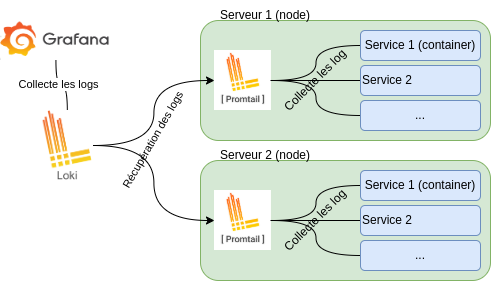
\includegraphics[scale=0.7]{./ressource/loki_Protmail.png}
\end{center}


\section{Pré-requis}
Pour effectuer le test de logs dans les meilleurs conditions, il est nécessaire de stopper les containers des tests précédents. Pour cela, soit vous allez dans \textbf{tous les répertoires} contenant vos \verb?docker-composee.yml? et vous taper la commande 
\begin{lstlisting}[style=commande]
sudo docker compose down
\end{lstlisting}

\vspace*{0.5cm}

Soit vous taper juste la commande suivante. Elle arrête tous les containers \textbf{Attention si vous en avez d'autres qui ne doivent pas être arrêtes}.
\begin{lstlisting}[style=commande]
sudo docker stop $(sudo docker ps -q)
\end{lstlisting}


\vspace*{0.5cm}

Normalement la commande pour visualiser les container lancés ne retourne rien

\begin{lstlisting}[style=commande]
$ sudo docker ps
CONTAINER ID   IMAGE     COMMAND   CREATED   STATUS    PORTS     NAMES
\end{lstlisting}


\paragraph{Service à scruter} \

Pour les tests, les logs des \textbf{services LEMP en HTTP} (non sécurisé) vont être collectés. Il est donc ncéessaire de le relancer. 
Pour rappel : 
\begin{itemize}
\itemE L'URL du dépôt est  : \url{https://github.com/PierreViland/00-serveurLemp.git}

\begin{center}
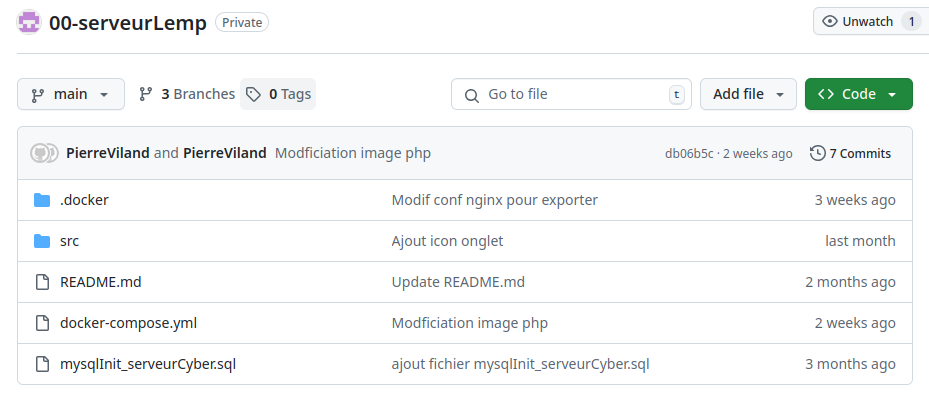
\includegraphics[scale=0.4]{./ressource/gitlamp}
\end{center}

\itemE La branche a utilisé est : \verb?main?
\begin{lstlisting}[style=commande]
$ git switch main
Already on 'main'
Your branch is up to date with 'origin/main'.
\end{lstlisting}

\itemE La commande pour l'ensemble l'ensemble des containers est : 
\begin{lstlisting}[style=commande]
$ sudo docker compose up -d
\end{lstlisting}


\end{itemize} 

\section{Eléments utilisés}

L'ensemble des éléments de configuration de la centralisation des logs est présent sur \textbf{ le même dépôt utilisé pour Prometheus} 
\begin{itemize}
\itemE \url{https://github.com/PierreViland/monitoringPV}
\itemE Avec le répertoire du dépôt \textbf{01-stackMonitoring} (déjà utilisé pour Prometheus)
\end{itemize}

\begin{center}
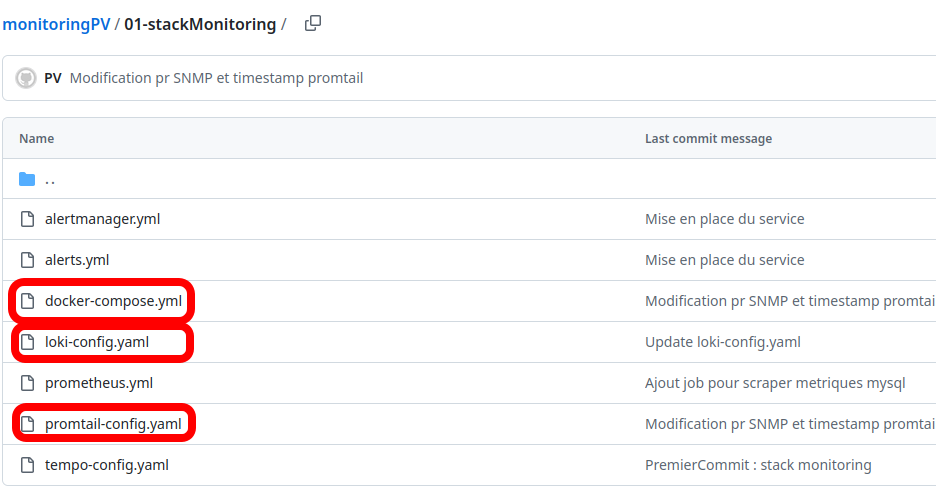
\includegraphics[scale=0.4]{./ressource/gitMonitoringPV}
\end{center}

Les trois ficheirs entourés vont être utilisé pour la gestion des logs : 
\begin{itemize}
\itemE \verb?docker-compose.yml? $\Rightarrow$ : Gestion et lancement des containers 
\itemE \verb?loki-config.yml? $\Rightarrow$ : Configuration de loki
\itemE \verb?promtail-config.yml? $\Rightarrow$  : Configuration de promtail
\end{itemize}



%\begin{center}
% \rule{0.5\linewidth}{1pt}
% \end{center}

 
 \section{Promtail}
 \subsection{Structure du fichier de configuration}
\textbf{Le fichier de configuration de promtail} se nomme \verb?promtail-config.yaml?. Il contient les éléments suivants qui peuvent être bien sûr modifier en fonction des besoins. 

\begin{center}
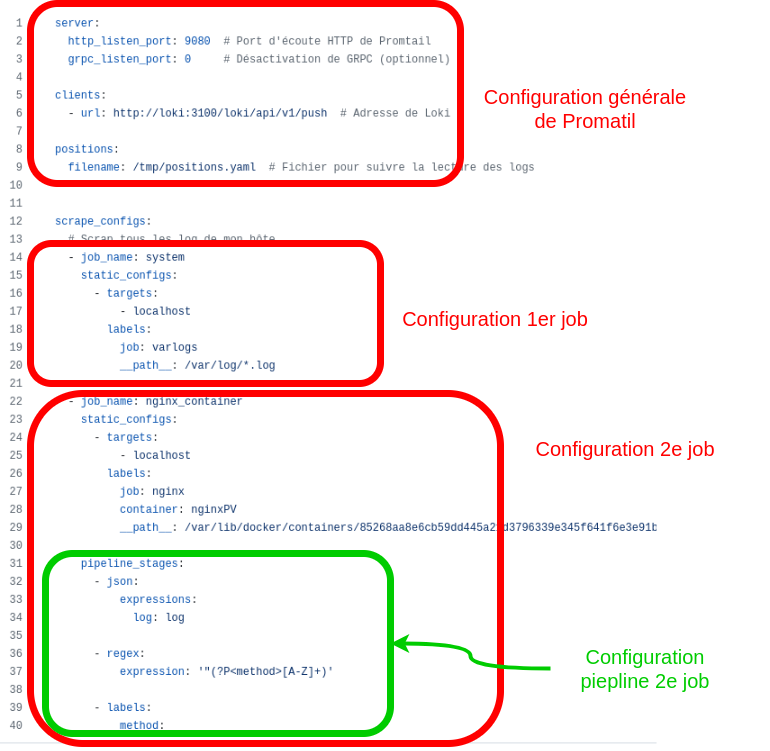
\includegraphics[scale=0.45]{./ressource/promtailConf.drawio.png}
\end{center}

\paragraph{Vocabulaire }
\begin{encadre}{Job dans Promtail}
Configuration de collecte des logs depuis une source spécifique (comme un fichier, syslog, journal, etc.), incluant le chemin des fichiers et les labels associés.
\end{encadre}

\begin{encadre}{Piepline dans Promtail}
Suite d'étapes de traitement (comme replace, json, regex, labeldrop) appliquées à chaque log pour l’extraire, le transformer ou enrichir les labels avant l’envoi à Loki.
\end{encadre}


\begin{encadre}{Label dans Promtail}
Paire clé-valeur attachée aux logs, utilisée pour filtrer, regrouper et acheminer les logs vers Loki. Ces labels facilitent la recherche et l'organisation des journaux dans Loki.
\end{encadre}


\paragraph{Détails de la configuration général}\ 



\begin{lstlisting}[style=commande]
server:
  http_listen_port: 9080
  grpc_listen_port: 0
\end{lstlisting}
avec : 
\begin{itemize}
\itemE  \verb? http_listen_port: 9080? : Promtail écoute sur le port 9080 pour l'interface HTTP.
\itemE  \verb?grpc_listen_port: 0? : Le port gRPC (Remote Procedure Call) est désactivé (valeur 0).
\end{itemize}

Ensuite on retrouve 
\begin{lstlisting}[style=commande]
clients:
  - url: http://loki:3100/loki/api/v1/push
\end{lstlisting}
qui spécifie où envoyer les logs. \verb?loki? est le nom du container (qui peut aussi être l'adresse IP) suivi de son port d'écoute \verb?3100?. Le reste de l'URL \verb?/loki/api/v1/push? ne peut pas être modifié.


Ensuite, il est précisé le nom du fichier utilisé pour suivre la position de lecture des logs (évite de tout relire à chaque démarrage).
\begin{lstlisting}[style=commande]
positions:
  filename: /tmp/positions.yaml
\end{lstlisting}

\textbf{Attention à modifier sous Windows}



\begin{center}
 \rule{0.5\linewidth}{1pt}
 \end{center}
\paragraph{Configuration des jobs}\ 

C'est ensuite que les différents \textbf{jobs} sont configurés permettant de dire à Promtail quels logs nous devons récupérer; Dans notre cas : 
\begin{itemize}
\itemE Logs de la machine hôte (serveur ubuntu)
\itemE Logs du container nginx
\end{itemize}



Dans cette exemple, le premier job récupère les logs du système hôte. \textbf{A modifier sous Windows}
\begin{lstlisting}[style=commande]
  # Scrap tous les log de mon hote
  - job_name: system
    static_configs:
      - targets:
          - localhost
        labels:
          job: varlogs
          __path__: /var/log/*.log
\end{lstlisting}

Ensuite, il est configuré la récupération des logs du container nginx  ayant pour ID \textbf{8526.....022d}. 
\begin{lstlisting}[style=commande]
- job_name: nginx_container

    static_configs:
      - targets:
          - localhost
        labels:
          job: nginx
          container: nginxPV
          __path__: /var/lib/docker/containers/85268aa8e6cb59dd445a21d3796339e345f641f6e3e91b7606b7d495c342022d/85268aa8e6cb59dd445a21d3796339e345f641f6e3e91b7606b7d495c342022d-json.log
\end{lstlisting}
La strucutre est similaire à la récupération des logs système : 
\begin{itemize}
\itemE \verb?target ? : représente le points de collecte.
\itemE \verb?job: nginx? : nom du job (qui sera utilisé par loki)
\itemE \verb?container: nginxPV ? : identifie le conteneurs 
\itemE \verb?__path__ ? : chemin exact du fichier de logs du conteneur.
\end{itemize}


\begin{center}
 \rule{0.5\linewidth}{1pt}
 \end{center}
\paragraph{Etage de pipeline}\ 

La suite des lignes est toujours relative au job \verb?nginx_container?. On y retrouve les \textbf{pipeline\_stages} qui sont des étapes de traitements des logs avant d'envoyer à loki. 


\begin{lstlisting}[style=commande]
    pipeline_stages:
  - json:
      # Extraction du champ 'log' depuis la ligne de log en format JSON
      expressions:
        log: log

  - regex:
      # Extraction de la methode HTTP (ex: GET, POST) depuis la chaine entre guillemets
      expression: '"(?P<method>[A-Z]+)'

  - regex:
      # Extraction de la date/heure au format specifique entre crochets dans 'log'
      expression: '\[(?P<date>\d{2}\/[A-Za-z]{3}\/\d{4}:\d{2}:\d{2}:\d{2} [+\-]\d{4})\]'
      source: log

  - timestamp:
      # Conversion de la date extraite en timestamp utilisable par Promtail
      source: date
      format: "02/Jan/2006:15:04:05 -0700"

  - labels:
      # Ajout du label 'method' pour filtrage et classification dans Loki
      method:
\end{lstlisting}


Comme nous le verrons dans la suite du document, les labels permettent des rechercher efficacement dans \textbf{loki}. Attention, un nombre trop important d'éléments dans un label risque d'impacter les performances de loki. 



\subsection{Le lancement d'un container Promtail}
 doit se faire sur chaque serveur. Les lignes du fichier \verb?docker-compose.yml? sont les suivantes : 

\begin{lstlisting}[style=commande]
 55   promtail:
 56     image: grafana/promtail:latest
 57     container_name: promtail
 58     volumes:
 59       - /var/log:/var/log
 60       - /var/lib/docker/containers:/var/lib/docker/containers:ro        
 61       - ./promtail-config.yaml:/etc/promtail/config.yaml
\end{lstlisting}
avec : 
\begin{itemize}
\itemE \verb? - /var/log:/var/log? : volume partagé contant les logs de la machines hôte. \textbf{A modifier sous windows}
\itemE \verb? - /var/lib/docker/containers:/var/lib/docker/containers:ro   ? : volume partagé contenant les fichiers des containers
\itemE \verb?- ./promtail-config.yaml:/etc/promtail/config.yaml?  : fichier de configuration de promtail
\end{itemize}


%\begin{center}
% \rule{0.5\linewidth}{1pt}
% \end{center}
% 

\section{Mise en place de loki}

Pou rappel, \textbf{Loki} permet la centralisation des données. Les lignes du \verb?docker-compose.yml? relatives à son lancement sont : 
\begin{lstlisting}[style=commande]
 41   loki:
 42     image: grafana/loki:latest
 43     container_name: loki
 44     ports:
 45       - "3100:3100"
 46     command:
 47       - "-config.file=/etc/loki/local-config.yaml"
 48     volumes:
 49       - ./loki-config.yaml:/etc/loki/local-config.yaml
 50       - ./loki-data:/data       
 51     user: "1000:1000"
 52     networks:
 53       - mynet
\end{lstlisting}


Le fichier de configuration est présent dans le dépôt et se nomme \verb?loki-config.yaml?. Aucune modification de ce fichier est nécessaire pour faire fonctionner loki. Il faut juste bien vérifier que le port d'écoute de loki soit le 3100
pour être en accord avec la configuration de promtail.
\begin{lstlisting}[style=commande]
server:
  http_listen_port: 3100
\end{lstlisting}



\section{Grafana}




\paragraph{Connexion avec loki}
\textbf{Grafana} (outil déjà utilisé) va permette de visualiser les logs. La première étape de de créer \textbf{une connexion de Grafana a Loki}. 

\begin{center}
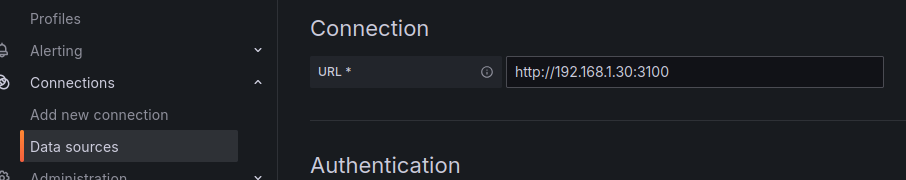
\includegraphics[scale=0.7]{./ressource/grafanRef_loki}
\end{center}
Dans le cas  ci-dessous, les logs sont récupérés via un container loki installé sur la machine \verb?192.168.1.30? en écoute sur le port \verb?3100?.


\paragraph{Explorer}


L'onglet Explore est une interface qui permet de consulter et analyser les logs en temps réel. Il est par exemple très facile de lister les log correspondant à une méthode GET ou une méthode POST. 
\begin{center}
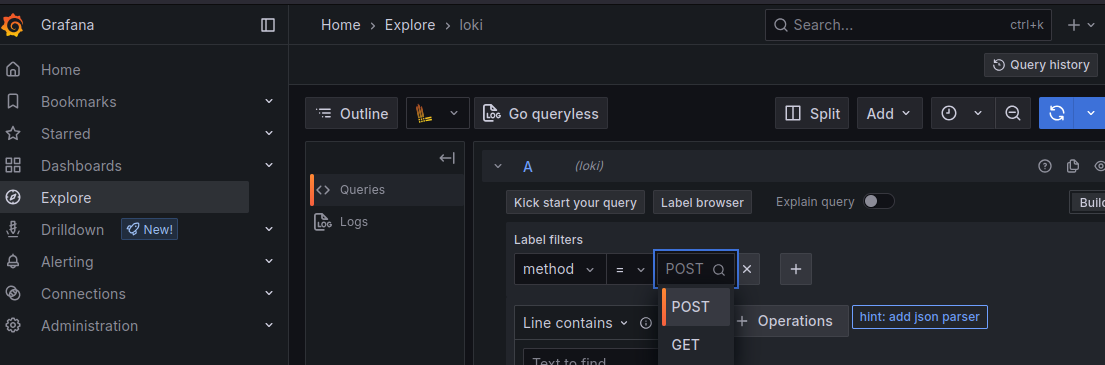
\includegraphics[scale=0.5]{./ressource/grafanaExplore}
\end{center}


\paragraph{Modification du dashbord}
Il est aussi possible de rajouter dans un dashbord le nombre de connexion GET (ou POST) par minute : 
\begin{lstlisting}[style=commande]
sum(count_over_time({job="nginx", method="GET"}[1m]))
\end{lstlisting}

\begin{center}
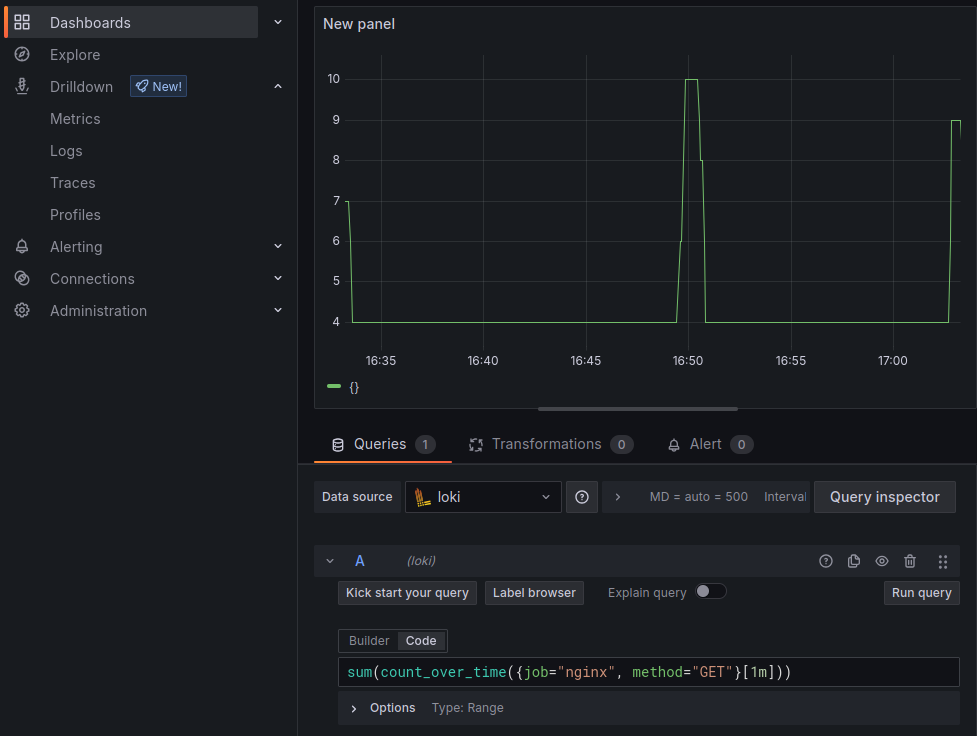
\includegraphics[scale=0.5]{./ressource/grafanaNombre_delelement.png}
\end{center}


\section{A faire avec les élèves}


L'avantage du service déployé est de fournir l'état de santé du système et du serveur. Il peut être intéressant d'avoir une vision détaillée de notre service web avec par exemple le nombre de codes HTTP. 

Pour rappel les codes sont : 

\begin{itemize}
\itemE \textbf{2xx} : succès
\itemE \textbf{3xx} : Redirection
\itemE \textbf{4xx} : erreurs côté client (ex. 404 page non trouvé)
\itemE \textbf{5xx} : erreurs serveur à surveiller en priorité (ex. 500, 502, 504)
\end{itemize}

\subsection{Erreur 404}

\begin{enumerate}
\item Trouver une erreur 404
\item Visualiser la sur grafana
\item Créer un dashboard sur Grafana qui permet de les visualiser. 
\end{enumerate}



\ifPROF
\color{red}
Essayer d'accéder à une page qui n'est pas référencé \verb.indexX.html?

Dans l'explorer, tester : 

\begin{lstlisting}[style=commande]
{container="nginxPV"} |= "HTTP" |~ " 404 "
\end{lstlisting}

et enfin dans un dashbord : 


	
\begin{lstlisting}[style=commande]
(count_over_time({container="nginxPV"} |= "HTTP" |~ " 404 "[1m]))
\end{lstlisting}

\begin{center}
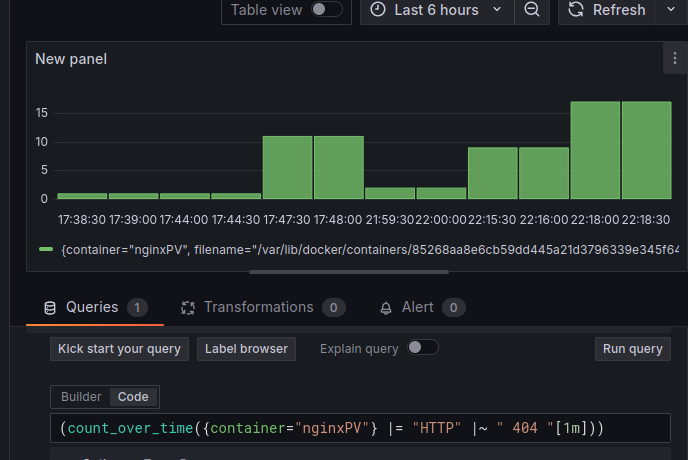
\includegraphics[scale=0.4]{./ressource/grafanaErreur404}
\end{center}
\normalcolor
\fi
\subsection{Erreur 5xx}

Idem a faire avec l'erreur 5xx qui est très sérieux car c'est un erreur interne serveur

\ifPROF
\color{red}
Le principe est le même que précdement mais il faudra modifier le serveur pour créer une erreur 500. Par exemple : 

\begin{itemize}
\itemE retour forcé via configuration Nginx
\end{itemize}

\begin{lstlisting}[style=commande]
location /error500 {
    return 500;
}
\end{lstlisting}
Puis, fais une requête sur /error500


\begin{itemize}
\itemE  Erreur 502 : Bad Gateway
\end{itemize}
Configure Nginx pour faire du reverse proxy vers un service qui n’existe pas ou qui ne tourne pas.

\begin{lstlisting}[style=commande]
location /error502 {
    proxy_pass http://localhost:9999;  # Port non utilisé volontairement
}
\end{lstlisting}

\normalcolor
\fi

\newpage
\section{Exemple réel}

Le système suivant a été mise en place. 

\begin{center}
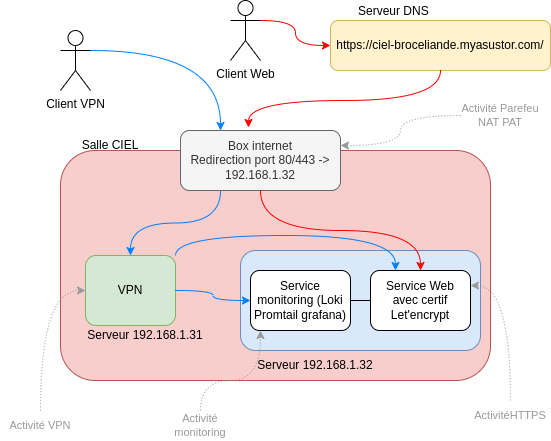
\includegraphics[scale=0.5]{./ressource/topoReseau.drawio.png}
\end{center}

Le serveur bleu d'adresse 192.168.1.32 est accessible 
\begin{itemize}
\itemE via l'url https://ciel-broceliande.myasustor.com/
\itemE via le serveur VPN présent dans la salle d'adresse 192.168.1.31. Des fichiers openvnp de configuration peuvent être fournis.
\end{itemize}
Il fournit 
\begin{itemize}
\itemE Un service web accessible en local et à l'extérieur 
\itemE Un service de monitoring accessible uniquement depuis le LAN
\end{itemize}

\vspace{0.25cm}
Pour se connecter à grafana, il faut dans un navigateur web utilisé l'URL suivant  
\begin{itemize}
\itemE \url{http://192.168.1.30:3000}
\end{itemize}


\vspace{0.25cm}
Les identifiants (peut sécurisé) : 
\begin{itemize}
\itemE login : \verb?admin?
\itemE mot de passe : \verb?acRennes!!2025?
\end{itemize}

\paragraph{Le dashboard} de monitoring du service web est le suivant : (il est amené à évolué en fonction des besoins

\begin{center}
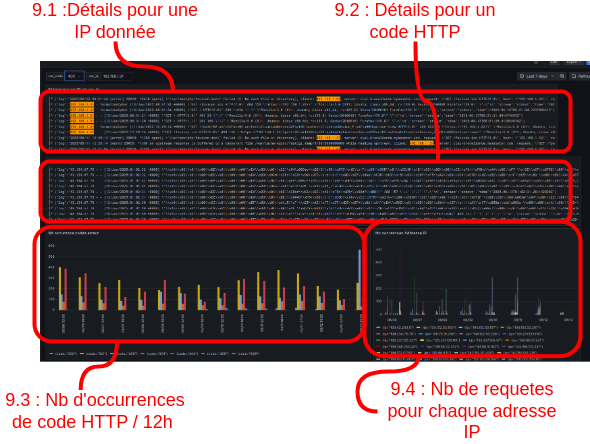
\includegraphics[scale=0.7]{./ressource/exempleRelle.drawio.png}
\end{center}

\subsection{Détails pour une IP Donnée}
Ce champs permet d'afficher tous les logs correspondant à une IP donnée. La commande logQL correspondante : 

\begin{lstlisting}[style=commande]
{container="nginxSecu"}
| regexp `(?P<ip>\d{1,3}(?:\.\d{1,3}){3})`
|= "$var_ip"
\end{lstlisting}

\paragraph{Avantage }
\begin{itemize}
\itemE Permet de regarder les logs d'une adresse IP suspecte
\end{itemize}

\subsection{Détails pour un code HTTP}

Ce champs permet de visualiser tous les logs correspondant à un code HTTP

\begin{lstlisting}[style=commande]
{container="nginxSecu", code=~"$var_code"}
\end{lstlisting}

\subsection{Nombre d'occurrence de code HTTP}

Ce champs montre le nombre d'occurrences des différents code HTTP par tranche de 12h

\begin{lstlisting}[style=commande]
sum by (code) (
  count_over_time({container="nginxSecu", code=~".+"}[1d])
)
\end{lstlisting}


\subsection{Nombre de requêtes pour chaque adresse IP}

Ce champs montre le nombre de requête pour chaque adresse ip par jour.

\begin{lstlisting}[style=commande]
sum by (ip) (
  count_over_time(
    {container="nginxSecu"}
    | regexp `(?P<ip>\d{1,3}(?:\.\d{1,3}){3})`
    | ip != ""
    | label_format ip="{{.ip}}"
  [1d])
)
\end{lstlisting}


\vspace{0.5cm}
Il est possible de limiter au 10 IP les plus actives

\begin{lstlisting}[style=commande]
topk(10,
  sum by(ip) (
    count_over_time(
      {container="nginxSecu"} 
        | regexp `(?P<ip>\d{1,3}(?:\.\d{1,3}){3})`
      [1d]
    )  ) )
\end{lstlisting}
\subsection{Filtrage couplé}

Il peut être intéressant d'effectuer un filtrage croisé pour voir les actions effectuée pas une adresse IP. 


\begin{center}
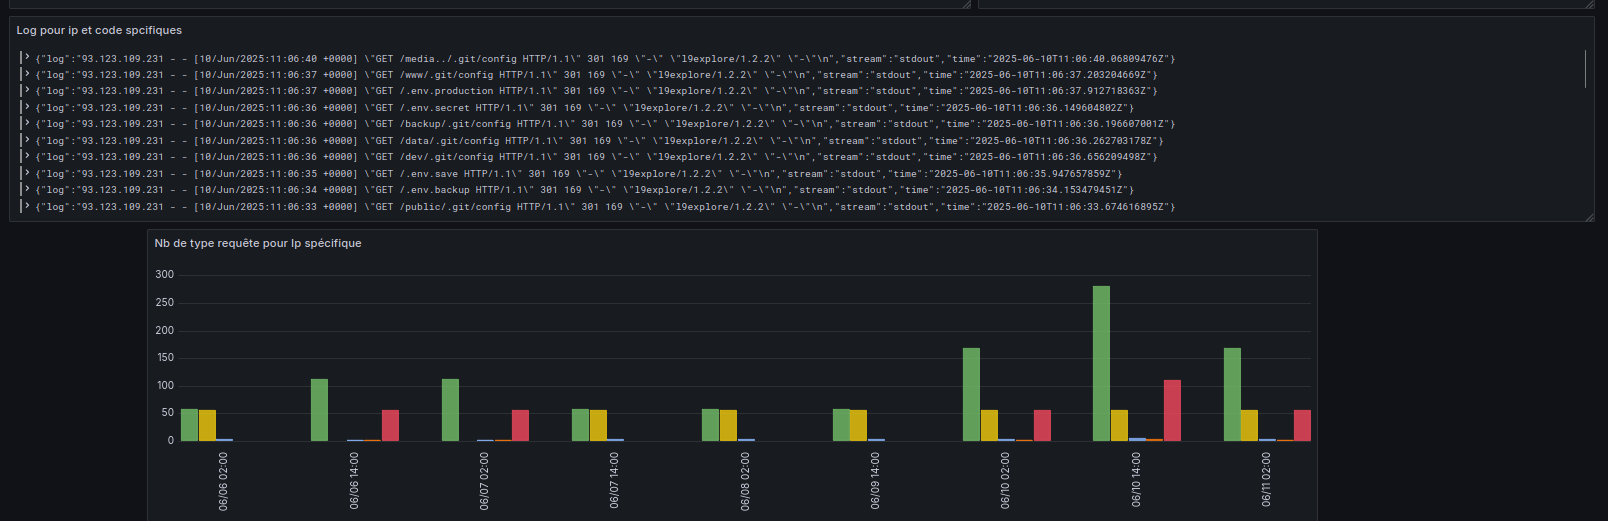
\includegraphics[scale=0.3]{./ressource/filtrageCroise}
\end{center}

Les 1re fenêtre permet de visualiser les logs filtré
\begin{itemize}
\itemE Pour une adresse IP
\itemE Pour un code d'erreur particulier
\end{itemize}

Le requête logQL est la suivante 
\begin{lstlisting}[style=commande]
{container="nginxSecu", code=~"$var_code"}
| regexp `(?P<ip>\d{1,3}(?:\.\d{1,3}){3})`
| ip=~"$var_ip"
\end{lstlisting}


\paragraph{La 2e fenêtre} permet de visualiser pour une adresse IP le nombre de code HTTP par demi journée.

\begin{lstlisting}[style=commande]
sum by (code) (count_over_time(
  {container="nginxSecu"}
  | regexp `(?P<ip>\d{1,3}(?:\.\d{1,3}){3})`
  | ip=~"$var_ip"
  [1d]
))
\end{lstlisting}


\subsection{Exemple d'activité}

\begin{itemize}
\itemE Les élèves ne mettent pas en place protmail mais loki et grafana sur leur machine
\itemE Ensuite il analyse les logs réelles. 

\itemE Ils en déduisent les mouvements et proposent des solutions (filtrage IP par exemple)
\end{itemize}





\end{document}